\textbf{Chapter 3}

\textbf{Methodology \& Mathematical Formulation}

This chapter explains how the portfolio problem can be treated as a
Markov Decision Process (MDP), i.e the trading process is treated as a
sequence of step-by-step decision-making problems. The objective is to
develop an environment in which an autonomous trading agent can learn an
optimal decision-making behaviour by interacting with a simulated
market. At each step, the portfolio system observes current market and
portfolio conditions, takes an action such as buying, selling, or
holding, receives a result based on how the portfolio's wealth changed,
and then moves to the next step.

The chapter then explains the two main learning methods used in the
project: \textbf{REINFORCE}---the Monte-Carlo policy gradient, which
learns by improving its strategy based on the rewards it receives ---and
\textbf{Deep Q-learning}, which learns which actions are likely to give
the best results. Finally, \textbf{PPO} is introduced as an additional
method in the ablation row to compare against the other approaches, as
it is designed to make the policy learning process more stable.

Table 3.1 collects every symbol used for reference.

\textbf{Table 3.1: Notation used throughout Chapters 3--5.}

{\def\LTcaptype{none} % do not increment counter
\begin{longtable}[]{@{}
  >{\raggedright\arraybackslash}p{(\linewidth - 2\tabcolsep) * \real{0.1885}}
  >{\raggedright\arraybackslash}p{(\linewidth - 2\tabcolsep) * \real{0.8115}}@{}}
\toprule\noalign{}
\begin{minipage}[b]{\linewidth}\raggedright
\textbf{Symbol}
\end{minipage} & \begin{minipage}[b]{\linewidth}\raggedright
\textbf{Meaning}
\end{minipage} \\
\midrule\noalign{}
\endhead
\bottomrule\noalign{}
\endlastfoot
\emph{s\textsubscript{t}} ∈ ℝ\textsuperscript{8} & state observed by the
agent at trading day t, containing the eight features used by the
trading system (Table 3.3) \\
\emph{a\textsubscript{t}} ∈ \{0, 1, 2\} & action selected by the agent:
Hold, Buy, or Sell. \\
\emph{P\textsubscript{t}} & asset price at day trading t; \\
\emph{r\textsubscript{t}} & reward received after an action, calculated
from the change in portfolio value after transaction costs. \\
\emph{C\textsubscript{t}} & amount of cash available to the agent at
trading day t \\
\emph{h\textsubscript{t}} & number of (fractional) units of the asset
held at trading day t. \\
\emph{W\textsubscript{t}} = \emph{C\textsubscript{t}} +
\emph{h\textsubscript{t}} \emph{P\textsubscript{t}} & Total portfolio
value, calculated as untouched cash plus the current value of the asset
held; \\
\emph{C\textsubscript{0}} & initial cash available at the beginning of
an episode. \\
\emph{c} & proportional transaction fee for taking a trade, set to
0.05\% (c = 0.05) \\
\emph{Δ} = 0.1 \emph{C\textsubscript{0}} & fixed monetary size of each
trade \\
\emph{γ} & discount factor used to determine the importance of future
rewards \\
\emph{τ} & a trajectory (one complete trading episode), corresponding to
one month of daily trading; related to \emph{t \& T} \\
\emph{T} & episode length in days (with 𝑇 ≈18--23) \\
\emph{t} & 1 trading day \\
\emph{G}(τ) & The total return obtained over a complete episode \\
\emph{G\textsubscript{t}} & The accumulated future reward from time t
onwards. \\
\emph{π\textsubscript{θ}}(\emph{a} \textbar{} \emph{s}) & policy network
that determines the likelihood of choosing action \emph{a} given the
current state \emph{s}. \\
\emph{Q\textsubscript{φ}}(s, \emph{a}) & The Q-network, which estimates
the value of taking a particular action in a given state; frozen target
copy \\
\emph{Q\textsubscript{φ⁻}} & A fixed copy of the Q-network used as a
target during Deep Q-learning. \\
\emph{J}(θ) & objective function representing the expected return of the
policy \\
\emph{ε} & exploration rate used by the (ε-greedy) action-selection
strategy \\
\end{longtable}
}

\textbf{3.1 Overview: Trading as a Markov Decision Process}

Reinforcement Learning (RL) trains an agent to make sequential decisions
by interacting with an environment. The environment is modelled as an
MDP where decisions are made at regular time steps, represented by the
tuple~\(\left( \mathcal{S},\mathcal{A},\mathcal{P},\mathcal{R},\gamma \right)\):
at step \(t\) the agent observes the current state \(s_{t} \in S\),
selects an action \(a_{t} \in A\), receives a numerical reward based on
the outcome \(r_{t}\), and the environment moves to the next state
\(s_{t + 1}\) according to the current state and the action selected by
the agent \(P(s_{t + 1}|s_{t},a_{t})\).

In this project, the trading environment is modelled in the same way,
providing a formal description of how the trading agent interacts with
the market over time; one time step \(t\) corresponds to one trading
day.

The state \(s_{t}\) represents all information available to the agent on
day \(t\) to fully capture its position within the trading episode. This
includes the selected market features, the agent\textquotesingle s
current portfolio position, and its available cash.

Based on this state, the agent selects one of three possible actions
\(a_{t} \in \left\{ 0,\ 1,\ 2 \right\}\): \emph{Hold the current
position, Buy a fixed amount, or Sell a fixed amount.} The selected
trade is then executed, with transaction fees \(c\) applied where
appropriate.

After taking an action, the environment calculates the change in the
agent\textquotesingle s total portfolio value and returns it as the
reward \(r_{t}\).

The environment advances to the next trading day \(s_{t + 1}\), and the
process repeats throughout the episode \emph{τ}, allowing the agent to
update its policy \(\pi_{\theta}\) or value estimates \(Q_{\phi}\) based
on the experience collected.

The interaction can therefore be represented as:
\(s_{t} \rightarrow a_{t} \rightarrow r_{t},s_{t + 1}\)

\textbf{Figure 3.1 illustrates the interaction between the trading agent
and the environment.}

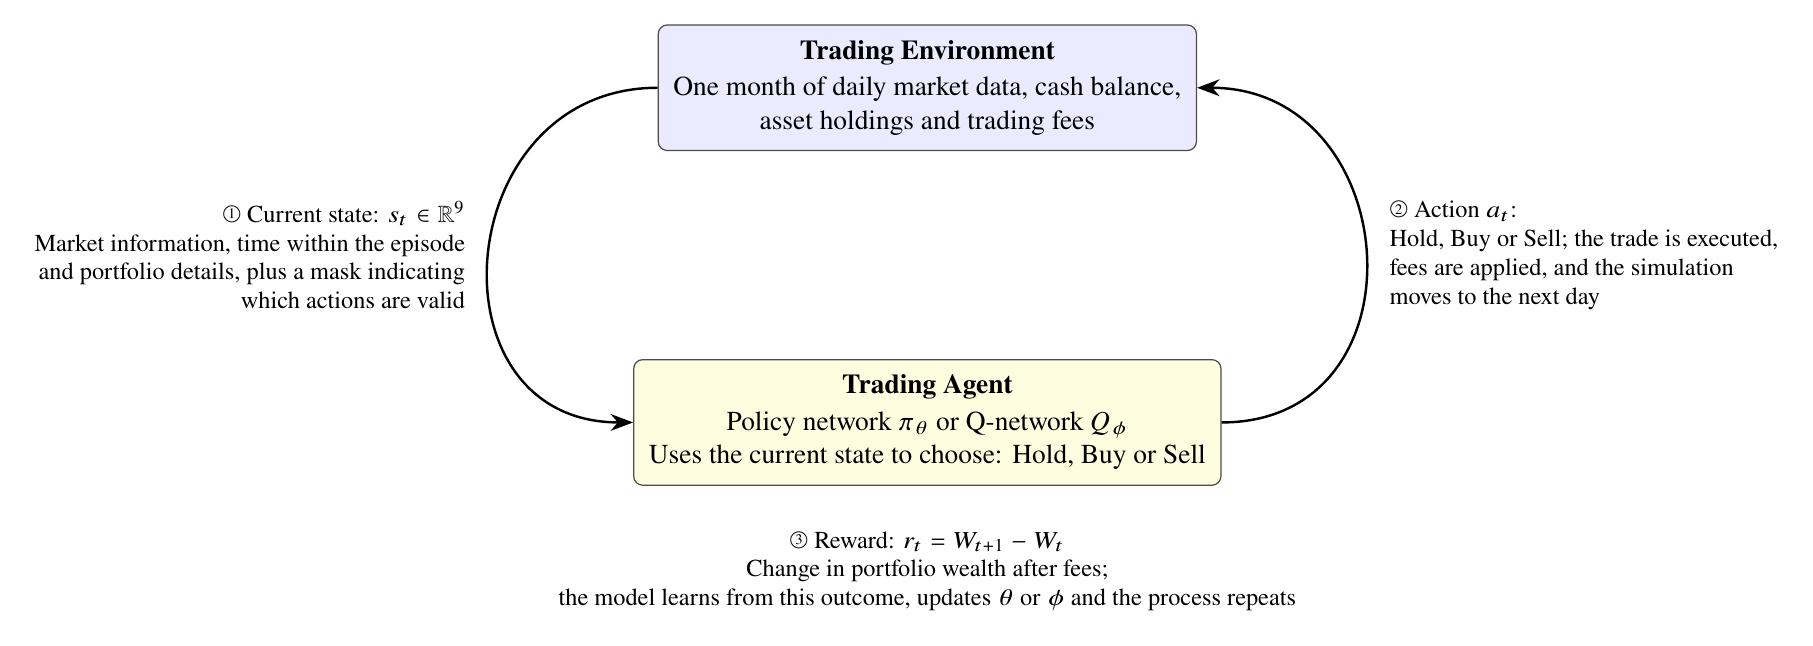
\includegraphics[width=6in,height=2.13789in]{media/media/image1_ch3.png}

Figure 3.1: The agent--environment interaction loop for the trading MDP.
One cycle corresponds to one trading day.

To make the MDP formulation easier to understand, Table 3.2 compares the
main components of the trading task with those of a familiar
game-playing task, Flappy Bird, which was used initially to understand
Reinforcement Learning.

\textbf{Table 3.2: Mapping a popular game MDP to the portfolio trading
MDP.}

{\def\LTcaptype{none} % do not increment counter
\begin{longtable}[]{@{}
  >{\raggedright\arraybackslash}p{(\linewidth - 4\tabcolsep) * \real{0.2129}}
  >{\raggedright\arraybackslash}p{(\linewidth - 4\tabcolsep) * \real{0.3872}}
  >{\raggedright\arraybackslash}p{(\linewidth - 4\tabcolsep) * \real{0.3998}}@{}}
\toprule\noalign{}
\begin{minipage}[b]{\linewidth}\raggedright
\textbf{MDP component}
\end{minipage} & \begin{minipage}[b]{\linewidth}\raggedright
\textbf{Flappy Bird}
\end{minipage} & \begin{minipage}[b]{\linewidth}\raggedright
\textbf{Trading (this work)}
\end{minipage} \\
\midrule\noalign{}
\endhead
\bottomrule\noalign{}
\endlastfoot
State \emph{s\textsubscript{t}} & Bird\textquotesingle s position and
speed, together with the position of the next pipe & Market information
and the agent\textquotesingle s current portfolio position \\
Action \emph{a\textsubscript{t}} & Flap or do not flap & Hold, Buy, or
Sell \\
Reward \emph{r\textsubscript{t}} & Survival score based on how long the
bird remains in play & Change in portfolio wealth after trading fees \\
Episode \emph{τ} & One complete game session & One calendar month of
daily trading \\
Terminal rule & The game ends when the bird crashes or hits the ground &
The episode ends at the final trading day, with any remaining position
sold \\
\end{longtable}
}

This analogy comparison also highlights an important design principle
used throughout the project. In Flappy Bird, the state sees the whole
world by containing enough information relevant to the next decision,
such as the bird\textquotesingle s position and movement and the
location of the pipes. The trading state follows the same principle by
including the relevant information available to the agent at each
trading step. This ensures the agent has access to the information it is
allowed to observe when making decisions, without being given future
information. Section 3.3 discusses the design of the trading state in
more detail.

\textbf{3.2 Episode Definition and Data Structure}

\textbf{3.2.1} \textbf{Episode definition} \(\mathbf{(\tau)}\)

Each episode \((\tau)\) represents one calendar month of daily closing
prices, from \(P_{0}\ to\ P_{T}\) \((P_{0},\ \ P_{1},\ldots,P_{T})\)
where \(T\) is typically between 18 and 23 trading days per month,
excluding public holidays when markets aren't open and weekends of
market inactivity \((T \approx 18 - 23)\). At the beginning of each
episode, the agent starts with cash and no asset holdings. It can then
trade throughout the month based on the available information. At the
end of the final trading day \(t\), any remaining position is
automatically sold. This ensures that no position is carried over from
one episode to the next.

\textbf{3.2.2} \textbf{Independence of Trading Episodes}

For the purposes of the experiment, each monthly episode is treated as a
separate and independent trading period. This is similar to treating
each game session in Flappy Bird as a separate episode.

However, this is a simplification because market conditions in
consecutive months are not truly independent. For instance, events and
trends in one month do influence the market in the following month. The
resulting data are therefore not independent over time.

Modelling these temporal relationships in greater detail would require
time-series or partially observable approaches, which are outside the
scope of this project. The implications of this assumption are discussed
further in the conclusion\textbf{.}

\textbf{3.2.3 Choice of Episode Length}

Monthly episodes were selected to provide a balance between the length
of each trading period and the total number of training examples
available.

A single year of daily data provides approximately 12 monthly episodes
and around 250 daily trading decisions. Using eight years of data from
2018 to 2025 gives 96 monthly episodes and approximately 2,000 daily
transitions. These episodes are divided chronologically into 58 months
for training and 38 months for testing. The data are not shuffled, which
prevents information from later periods from being used during training
and helps avoid look-ahead leakage.

The same environment could also be adapted to use minute-level data in
future work. A typical trading session \(T\) would contain approximately
\textasciitilde{} 390 one-minute intervals in this case, providing a
much larger number of possible decision points. This would not require a
fundamental change to the environment because the framework is designed
to work across different episode lengths. However, minute-level trading
is outside the scope of the current study and is therefore left as a
potential area for future development.

\textbf{3.2.4 Selection of the Historical Period}

The experiments use daily market data from 2018 to 2025 as a fixed
period. Earlier data, including data from 2016 and before, were not
included in the main experimental period because the study aims to
evaluate the learning algorithms under relatively recent and varied
market conditions. These selected periods contain a range of market
conditions, including relatively stable periods in 2018, the market
decline associated with the COVID-19 pandemic and its subsequent
recovery, the later period of increased inflation and interest rates,
and the war in Ukraine in 2022, which caused weaker market conditions.
As a result, the dataset is not limited to a single type of market
condition, providing a useful range for evaluating the behaviour of the
portfolios trading agents without extending the dataset into
substantially older market years.

The exclusion of earlier data does not imply that those years are
unsuitable for financial modelling. Instead, the decision was to keep
the experimental dataset focused and consistent with the
study\textquotesingle s scope. Including older data, such as 2016 or
earlier, would increase the number of observations but could also
introduce market conditions that differ considerably from those in the
selected period; for instance, older microstructure and fee regimes that
differ slightly.

Earlier historical data could therefore be considered in future work as
an additional robustness test to examine how well the trained agents
generalise across different historical market regimes.

\textbf{3.2.5 MDP Limitations}

Although the portfolio trading problem is modelled as an MDP, real
financial markets are much more complex and cannot be assumed to be
fully observable.

The Markov assumption means that the current state should contain all
the information the agent needs to make its next decision. In a real
market, however, many external factors can affect price movements that
are not directly available to the agent. These include:

\begin{itemize}
\item
  economic announcements;
\item
  investor sentiment;
\item
  order-book activity;
\item
  geopolitical events;
\item
  movements in related assets.
\end{itemize}

As a result, the MDP used in this dissertation should be viewed as a
simplified representation of the portfolio trading problem rather than a
complete model of how real financial markets operate.

The purpose of the state design is therefore not to capture every factor
that may influence an asset\textquotesingle s price, but to provide the
agent with the key information needed to make decisions within the
controlled trading environment used for the experiments.

\textbf{3.3 State Representation Design}

In reinforcement learning, how information is presented to the agent
plays an important role in the quality of decisions it can learn. The
state representation must provide enough information for the agent to
understand the current situation and choose an appropriate action.

In this portfolio trading problem, this requires capturing information
about both the market and the agent\textquotesingle s own portfolio. The
agent needs to know how the asset has been moving, but it also needs to
know how much cash is available, whether it currently holds the asset,
whether that position is profitable, and how much time remains before
the trading period ends.

A state that leaves out important information can make it difficult for
the agent to learn effective strategies, even if the learning algorithm
is suitable for the task. This is because the agent can make decisions
only using the information provided. Therefore, the state representation
in this study was developed gradually by first examining simpler
representations and then adding information as needed to address
specific limitations of the previous representation.

The objective was not to create an unnecessarily complex state
representation with many variables, but to design a compact
representation containing all relevant information needed for
decision-making within the defined portfolio trading environment, while
avoiding features that simply duplicate information already available
from other variables

\textbf{3.3.1 Information Available to the Agent}

As discussed in Section 3.1, the state should see the whole by providing
the agent with information relevant to its decision, as the Flappy Bird
state does. In a trading environment, this information can be divided
into two halves: \textbf{the agent\textquotesingle s own portfolio} and
\textbf{the wider market}. These two areas behave very differently and
should therefore be considered separately when designing the state.

The first area is the agent\textquotesingle s own portfolio. This
includes information such as the amount of cash available, how much of
the asset it owns, what it paid to enter a trade position, and the time
remaining in the trading period. The agent controls this half; it is not
hidden or estimated, and it can be completely represented. Given the
sequence of the asset prices and the agent\textquotesingle s actions,
the portfolio can be updated directly using the trading environment's
rules.

The second area is the market. Here, complete information about the
market is impossible in principle and cannot be provided to the agent
because many factors affecting an asset's price are not directly
observable from the available price data. For example, the agent cannot
observe other market participants\textquotesingle{} decisions,
expectations, or intentions. Similarly, information such as news, market
sentiment, and macroeconomic events may influence prices without
appearing directly in the closing price at the end of the episode.

Adding more features calculated from past prices can give the agent
additional information about recent market behaviour, but it cannot
reveal everything happening in the market, as the future remains only
partly predictable from them. Future price movements therefore remain
uncertain, even when a relatively large number of historical features
are included.

The Flappy Bird analogy therefore needs some qualification, as its world
is finite and deterministic, so a handful of numbers genuinely is
sufficient. A market's world is neither. The attainable goal is a state
representation that is complete on the agent\textquotesingle s portfolio
side and rich enough on the market side that adding further features no
longer changes what the agent does.

For this reason, the state representation used in this study makes an
important note. \textbf{The portfolio information can be represented
completely because the environment directly controls and records it,
whereas market information can only approximate the wider market.}

Whether the additional market features provide useful information is
ultimately an empirical question, which is considered when evaluating
the state representation later in the dissertation.

\textbf{3.3.2 Criteria for a Suitable Trading State}

It is tempting to design a state by asking which features look useful,
but this is a weak approach as it says nothing about whether the object
being trained is an MDP at all.

Before deciding on the final state representation, three conditions were
considered. These provide a basis for deciding whether the proposed
state contains the information required for the portfolio trading
problem.

\textbf{1. Reward measurability}

The reward should be calculable from information available to the agent
and the resulting transition. If the reward depends on information not
contained in the state or the transition, the agent is effectively being
evaluated using information it cannot observe.

The primary reward used in this study is based on the change in
portfolio wealth:

\[r_{t} = W_{t + 1} - W_{t}\]

where:

\[W_{t} = C_{t} + h_{t}P_{t}\]

Here, \(C_{t}\) represents the available cash,

\(h_{t}\) represents the number of asset units held, and

\(P_{t}\) represents the current asset price.

To make these values comparable across different starting capital
levels, the final state uses normalised cash and asset exposure:

\[c_{t} = \frac{C_{t}}{C_{0}}\]

and:

\[v_{t} = \frac{h_{t}P_{t}}{C_{0}}\]

where \(C_{0}\) represents the initial capital.

These two features can be combined as:

\[c_{t} + v_{t} = \frac{C_{t}}{C_{0}} + \frac{h_{t}P_{t}}{C_{0}} = \frac{W_{t}}{C_{0}}\]

This means the agent\textquotesingle s current portfolio wealth,
relative to its initial capital, can be obtained directly from the
state, ensuring the reward can be calculated from the observed
transition without relying on information or variables hidden from the
agent.

Consequently, the wealth-change reward can be written as:

\[W_{t} = C_{0}\lbrack c_{t} + v_{t}\rbrack\]

\[r_{t} = C_{0}\left\lbrack \left( c_{t + 1} + v_{t + 1} \right) - \left( c_{t} + v_{t} \right) \right\rbrack\]

The reward can therefore be calculated from the current state, action,
and next state \({(s}_{t},\ a_{t},s_{t + 1})\) with no additional hidden
portfolio variable.

\textbf{2. Transition consistency}

The state should also contain enough information for the next state to
be determined from the current state, the selected action, the next
observed market price, and the trading environment rules.

This matters because the agent should not need to access hidden
historical variables to describe how its portfolio changes after an
action.

For example, the current portfolio exposure can be used to determine the
position's value, while the current unrealised profit/loss contains
information about the position\textquotesingle s entry price. Together
with the current price and the environment\textquotesingle s trading
rules, these quantities provide the information required to update the
portfolio after an action.

This keeps the state representation consistent with the defined trading
environment rather than requiring the environment to retrieve additional
portfolio history that is not represented in the state.

\textbf{3. Decision sufficiency}

The state should contain enough information for the agent to make a
decision based on the current trading situation without ambiguity. If
two different situations look identical to the agent but require
different actions, then the state is missing important information,
making the representation incomplete.

For example, consider the following two situations:

\begin{itemize}
\item
  the asset price has increased by 2\% today, and the agent does not
  hold the asset;
\item
  the asset price has increased by 2\% today, but the agent holds a
  position that is currently making a loss.
\end{itemize}

In both cases, the observed price movement is the same. However, the
most appropriate action may be different. In the first situation, the
agent may consider opening a position, whereas in the second, it may
consider reducing or closing its existing position to minimize its
losses.

The state representation must therefore include information about both
the market and the agent\textquotesingle s own portfolio.

\textbf{3.3.3 Development of the State Representation}

The initial state representation included only basic information about
market movement and the agent's portfolio. While this provides a simple
starting point, it does not give the agent enough context to fully
understand its trading situation.

For instance, recent price changes alone do not tell the agent whether
it owns the asset, how much capital remains available, or whether an
existing position is in a profit or loss. Without this information, the
agent may interpret the same market condition in the same way, even when
the appropriate action depends on its current portfolio situation.

To address this limitation, the state representation was gradually
expanded in multiple stages. Each stage introduced additional
information to address a specific weakness identified in the previous
representation.

\textbf{3.3.3.1 Stage 1: Price-only representation}

The first and simplest representation provided the agent with only the
recent return of the asset:

\[s_{t}^{(0)} = \left\lbrack \Delta P_{t} \right\rbrack\]

where:

\[\Delta P_{t} = \frac{P_{t} - P_{t - 1}}{P_{t - 1}}\]

This feature represents the immediate change in the asset price between
two consecutive time steps.

However, this representation is insufficient because the same market
movement can lead to different trading situations. For example, a
positive daily return in price could occur in two different situations:

\begin{itemize}
\item
  the agent does not currently hold the asset and may consider entering
  a position;
\item
  the agent already holds a large position and may consider reducing its
  exposure.
\end{itemize}

Although the market information is identical in both cases, the most
suitable action may be different. The first limitation of the state is
therefore that the agent cannot see its own portfolio.

This highlights the need for the state representation to include
information about the agent's own portfolio state in addition to market
movement.

\textbf{3.3.3.2 Stage 2: Portfolio-aware representation}

The second representation extends the state by including basic
information about the agent's portfolio:

\[s_{t}^{(1)} = \left\lbrack \Delta P_{t},\ C_{t},\ h_{t} \right\rbrack\]

where:

\begin{itemize}
\item
  \(\text{(}C_{t})\) represents the amount of available cash in the
  portfolio;
\item
  \(\text{(}h_{t}\text{)}\) represents the number of asset units
  currently held in the portfolio.
\end{itemize}

By including portfolio information, the agent can distinguish between
different portfolio situations and make decisions based on its available
resources. For example, it can identify whether it has enough capital to
open a new position or whether it already holds the asset.

However, this representation is still incomplete. The number of units
held alone does not fully describe the financial size of the current
position. For instance, holding ten units of an asset has a very
different financial impact when the asset price is £10 compared with
when it is £1,000.

Furthermore, the agent cannot also determine whether its current
position is profitable because it does not know the purchase price. It
also lacks information on how much time remains in the trading episode
ends, which may influence decision-making.

Therefore, further information is required to create a more complete
representation of the agent's trading environment.

\textbf{3.3.3.3 Stage 3: Position-aware representation}

To address the limitations of the previous representation, the state was
extended to include information about the size of the current position
opened and its performance. This allows the agent to better understand
what it owns and the financial impact of its current position.

The following variables were added:

\[s_{t}^{(2)} = \left\lbrack \Delta P_{t},c_{t},v_{t},PnL_{t} \right\rbrack\]

\textbf{1. Normalised cash} \(\mathbf{(c}_{\mathbf{t}}\mathbf{)}\)

\[c_{t} = \frac{C_{t}}{C_{0}}\]

where \(C_{t}\) represents the available cash in the portfolio at time
\(t\), and

\(C_{0}\) represents the portfolio\textquotesingle s initial capital.

This feature indicates the proportion of the original capital that
remains available for future decisions. By using a normalised value, the
information remains consistent regardless of the starting account size.

\textbf{2. Normalised exposure} \(\mathbf{(v}_{\mathbf{t}}\mathbf{)}\)

\[v_{t} = \frac{h_{t}P_{t}}{C_{0}}\]

This represents the current market value of the open position relative
to the initial capital.

This gives the agent a clearer understanding of its actual asset
exposure, unlike simply recording the number of units held. For example,
the same number of units can represent a small or large investment
depending on the current asset price.

The normalised cash and asset exposure can also be combined to estimate
the agent's current wealth:

\[c_{t} + v_{t} = \frac{W_{t}}{C_{0}}\]

where \(W_{t}\) represents the current portfolio wealth.

This allows the agent to reconstruct its current wealth from the cash
available, and the value of the asset currently held in the portfolio.

\textbf{3. Unrealised profit/loss}
\(\mathbf{(Pn}\mathbf{L}_{\mathbf{t}}\mathbf{)}\)

\[PnL_{t} = \frac{P_{t} - {\overline{P}}_{t}^{entry}}{{\overline{P}}_{t}^{entry}}\]

Where \({\overline{P}}_{t}^{entry}\) represents the average price at
which the current position was opened.

This feature allows the agent to identify whether its current position
is profitable or losing. Without this information, the agent cannot
distinguish between different situations that look identical from a
market perspective.

For example, holding an asset after a price increase may be profitable
if the asset was purchased at a lower price. However, holding the same
asset could instead be losing money if the position was entered at a
higher price before the price declined.

Including unrealised profit/loss enables the agent to recognise this
difference and make more informed decisions.

\textbf{3.3.3.4 Stage 4: Time-aware representation}

Trading decisions are also affected by the amount of time remaining
within the trading episode

In this environment, each episode represents a fixed trading period,
meaning that all open positions must be closed before the final
timestep. Therefore, an action may have different consequences depending
on when it is taken.

For example, buying an asset at the start of an episode gives the
position more time to potentially increase in value compared with buying
the same asset shortly before the episode ends, when the position must
soon be closed.

To capture this information, the state representation includes the
remaining time left in the episode:

\[s_{t}^{(3)} = \left\lbrack {\Delta P_{t}}_{t},c_{t},v_{t},PnL_{t},\tau_{t} \right\rbrack\]

\[\tau_{t} = \frac{t}{T}\]

Where \(T\) represents the total length of the trading episode.

A value close to 0 indicates that the episode has only recently started,
while a value close to 1 indicates that the end of the episode is
approaching.

This feature lets the agent to take the remaining trading episode into
account when selecting an action and adjust its decisions accordingly.
For example, the agent may be more willing to take long-term positions
early in the episode, while becoming more cautious as the final timestep
approaches.

\textbf{3.3.4 Final State Representation}

Although the previous stages successfully introduced information about
the agent's portfolio and position, they provide limited understanding
of the broader market conditions. A trading decision should not depend
only on the most recent price change, as different market situations
exist, producing similar short-term movements.

For this reason, the agent also needs information that helps identify
the current market conditions to be able to distinguish between them,
such as:

\begin{itemize}
\item
  whether the asset is experiencing a short-term upward or downward
  trend;
\item
  whether the market is currently stable or highly volatile;
\item
  whether the current price is above or below its recent average level.
\end{itemize}

Therefore, additional market-related features are included to give the
agent a more complete view of the trading environment.

The final state representation is defined as:

\[\boxed{s_{t}^{(4)} = \left\lbrack \Delta P_{t},mom_{t},vol_{t},gap_{t},{rng_{t},\tau}_{t},c_{t},v_{t},PnL_{t} \right\rbrack \in \mathbb{R}^{9}}\]

The following variables were added:

\textbf{1. Momentum}

\[mom_{t} = \frac{P_{t} - P_{t - k}}{P_{t - k}}\]

Where \(k = 5\) previous days \textasciitilde{} 1 week timestep

Momentum measures the direction of price movement over the previous five
timesteps. It gives the agent a longer view of recent price direction
and helps the agent differentiate between a temporary price movement
from a more consistent trend developing over several timesteps.

\textbf{2. Volatility}

\[vol_{t} = \sigma\left( \Delta P_{t - k + 1},...,\Delta P_{t} \right)\]

Where \(\sigma\) represents the standard deviation of recent returns and
\(k = 5\).

Volatility measures how much recent returns have varied using Standard
Deviation.

This feature helps the agent recognise differences in market
uncertainty. For example, a 2\% price increase during a relatively
stable period is different from a 2\% increase during a period of large
and frequent price movements, indicating a riskier situation.

\textbf{3. Price trend position}

\[gap_{t} = \frac{P_{t}}{MA_{m,t}(P)_{t}} - 1\]

where \({MA}_{m,t}(P)_{t}\) represents the simple moving average of the
asset's closing price over the previous \((m = 20)\) days
\textasciitilde{} 1-month timesteps.

The simple moving average \({MA}_{m,t}(P)_{t}\) can be calculated as:

\[{MA}_{m,t}(P)_{t} = \frac{1}{m}\sum_{i = 0}^{m - 1}P_{t - i}\]

This feature shows whether the current price is above or below its
recent average. A positive value indicates that the current price is
above its recent average level, while a negative value indicates that it
is below it, helping the agent identify potential trends or deviations
from normal price behaviour.

\textbf{4. Normalised Trading Range}

The normalised trading range is based on the Average True Range (ATR):

\[rng_{t} = \frac{ATR_{n,t}}{P_{t}}\]

The True Range at timestep \(t\) is:

\[TR_{t} = \max\left( H_{t} - L_{t},\,\left| H_{t} - C_{t - 1} \right|,\,\left| L_{t} - C_{t - 1} \right| \right)
\]where:

\begin{itemize}
\item
  \(H_{t}\) = current high price
\item
  \(L_{t}\)= current low price
\item
  \(C_{t - 1}\)= previous closing price
\end{itemize}

The ATR is then calculated from the recent True Range values. Using the
simple rolling arithmetic mean procedure, the calculation after the
initial \((n = 14)\) days \textasciitilde{} 2-week timesteps value can
be expressed as:

\[ATR_{n,t} = \frac{1}{n}\sum_{i = 0}^{n - 1}TR_{t - i}\]

\[ATR_{14,t} = \frac{1}{14}\sum_{i = 0}^{13}TR_{t - i}\]

The \emph{Average True Range (ATR)} measures the size of recent price
movement using the asset's highest price point, lowest price point, and
closing prices. Dividing the ATR by the current price creates a
normalised measure, making it easier to compare price movements across
different price levels.

The features are organised into four categories:

\textbf{Table 3.3a: Feature Categorization}

{\def\LTcaptype{none} % do not increment counter
\begin{longtable}[]{@{}
  >{\raggedright\arraybackslash}p{(\linewidth - 4\tabcolsep) * \real{0.2565}}
  >{\raggedright\arraybackslash}p{(\linewidth - 4\tabcolsep) * \real{0.2629}}
  >{\centering\arraybackslash}p{(\linewidth - 4\tabcolsep) * \real{0.4773}}@{}}
\toprule\noalign{}
\begin{minipage}[b]{\linewidth}\centering
\textbf{Category}
\end{minipage} & \begin{minipage}[b]{\linewidth}\centering
\textbf{Features}
\end{minipage} & \begin{minipage}[b]{\linewidth}\centering
\textbf{Purpose}
\end{minipage} \\
\midrule\noalign{}
\endhead
\bottomrule\noalign{}
\endlastfoot
Market behaviour & \(\Delta P_{t},mom_{t},vol_{t},gap_{t}\) & Describe
recent market conditions and price behaviour \\
Portfolio information & \(c_{t},v_{t}\) & Describe available capital and
current exposure \\
Position information & \(PnL_{t}\) & Describe performance of any
position opened \\
Time information & \(\tau_{t}\) & Represent the remaining trading
episode \\
\end{longtable}
}

\textbf{Table 3.3b: Full State Definition}

\emph{Table 3.3b: The} \emph{nine-feature state representation
(s\textsubscript{t} ∈ ℝ\textsuperscript{9}) used in the main
experiments. C\textsubscript{0} denotes the initial cash,
h\textsubscript{t} the number of asset units held, and
W\textsubscript{t} = C\textsubscript{t} + h\textsubscript{t}
P\textsubscript{t} the portfolio wealth at time t. the mark-to-market
wealth. The feature timestep lengths are set to (k=5) for momentum and
volatility, (m=20) for the moving-average reference, and (n=14) for the
Average True Range.}

{\def\LTcaptype{none} % do not increment counter
\begin{longtable}[]{@{}
  >{\raggedright\arraybackslash}p{(\linewidth - 6\tabcolsep) * \real{0.0521}}
  >{\raggedright\arraybackslash}p{(\linewidth - 6\tabcolsep) * \real{0.1159}}
  >{\raggedright\arraybackslash}p{(\linewidth - 6\tabcolsep) * \real{0.2666}}
  >{\raggedright\arraybackslash}p{(\linewidth - 6\tabcolsep) * \real{0.5653}}@{}}
\toprule\noalign{}
\begin{minipage}[b]{\linewidth}\raggedright
\textbf{\#}
\end{minipage} & \begin{minipage}[b]{\linewidth}\raggedright
\textbf{Feature}
\end{minipage} & \begin{minipage}[b]{\linewidth}\raggedright
\textbf{Definition}
\end{minipage} & \begin{minipage}[b]{\linewidth}\raggedright
\textbf{What it tells the agent}
\end{minipage} \\
\midrule\noalign{}
\endhead
\bottomrule\noalign{}
\endlastfoot
\multicolumn{4}{@{}>{\raggedright\arraybackslash}p{(\linewidth - 6\tabcolsep) * \real{1.0000} + 6\tabcolsep}@{}}{%
\emph{\textbf{Market}}} \\
1 & \emph{ΔP\textsubscript{t}} & \emph{P\textsubscript{t}} -
\emph{P\textsubscript{t−1}}/ \emph{P\textsubscript{t−1}} & The most
recent price movement \\
2 & \emph{mom\textsubscript{t}} & \emph{P\textsubscript{t}} -
\emph{P\textsubscript{t−k}}/ \emph{P\textsubscript{t−k}} & whether that
recent price movement is part of a short-term trend \\
3 & \emph{vol\textsubscript{t}} &
\(\sigma\left( \Delta P_{t - k + 1},...,\Delta P_{t} \right)\) & how
much the asset price has been varying recently \\
4 & \emph{gap\textsubscript{t}} & \emph{P\textsubscript{t}} /
MA\emph{\textsubscript{m}}(P) − 1 & how far the current price is from
its recent average \\
5 & \emph{rng\textsubscript{t}} & ATR\emph{\textsubscript{n}}(P) /
\emph{P\textsubscript{t}} & The size of the recent price ranges, which
closing prices alone cannot show \\
\multicolumn{4}{@{}>{\raggedright\arraybackslash}p{(\linewidth - 6\tabcolsep) * \real{1.0000} + 6\tabcolsep}@{}}{%
\emph{\textbf{Portfolio}}} \\
6 & \emph{c\textsubscript{t}} & \emph{C\textsubscript{t}} /
\emph{C\textsubscript{0}} & how much of the initial cash remains
available as cash \\
7 & \emph{v\textsubscript{t}} & \emph{h\textsubscript{t}}
\emph{P\textsubscript{t}} / \emph{C\textsubscript{0}} & The current
value of the open position relative to the initial capital \\
\multicolumn{4}{@{}>{\raggedright\arraybackslash}p{(\linewidth - 6\tabcolsep) * \real{1.0000} + 6\tabcolsep}@{}}{%
\emph{\textbf{Position}}} \\
8 & \emph{PnL\textsubscript{t}} & (\emph{P\textsubscript{t}} −
\emph{P̄\textsubscript{tentry}}) / \emph{P̄\textsubscript{tentry}} &
whether the open positions are in profit or loss \\
\multicolumn{4}{@{}>{\raggedright\arraybackslash}p{(\linewidth - 6\tabcolsep) * \real{1.0000} + 6\tabcolsep}@{}}{%
\emph{\textbf{Time}}} \\
9 & \emph{τ\textsubscript{t}} & \emph{t} / \emph{T} ∈ {[}0, 1{]} & how
much time remains before the trading episode ends \\
\end{longtable}
}

\textbf{3.3.5 Feature Redundancy and Excluded Information}

The state was not designed by adding every potentially useful market
indicator. Features were included only where they provide information
that cannot already be recovered from the other variables in the state.

This is important because adding a feature that simply repeats existing
information increases the size of the input without providing the agent
with anything new.

The following features were excluded:

\textbf{1. Running portfolio return}

For example, the portfolio\textquotesingle s current return relative to
its starting capital\\
does not need to be included as a separate feature because it can
already be calculated from normalised cash and asset exposure:

\[c_{t},v_{t - 1}\]

Therefore, adding running portfolio return would duplicate information
already available in the state.

\textbf{2. Raw position size}

The raw number of units held, \(h_{t}\), is also not included in the
final state. The financial value of the position is more directly
represented by:

\[v_{t} = \frac{h_{t}P_{t}}{C_{0}}\]

This provides information about the actual exposure rather than only the
number of units.

\textbf{3. Raw asset price}

The raw asset price is also not required as a separate feature. The
state instead uses returns and normalised values, which describe price
movements without depending on the standard price level.

The general principle is therefore to include features that provide
useful information while avoiding variables that can already be
reconstructed from information available elsewhere in the state.

\textbf{3.3.6 The Risk-Aware Extension: Drawdown State}

The main state representation contains the information needed for the
change in wealth reward. However, it does not describe the history of
the portfolio's losses. This matters for risk-sensitive experiments
because the current portfolio value alone does not show how much the
portfolio may have fallen from a previous high.

This becomes important when considering losses and the
portfolio\textquotesingle s previous performance because current
portfolio wealth alone does not show how the portfolio reached its
current value. For example, two portfolios can have exactly the same
wealth at the current timestep but may have followed very different
paths:

\begin{itemize}
\item
  one portfolio may have increased steadily over time;
\item
  another may have suffered a large loss before recovering to the same
  level.
\end{itemize}

To address this, an additional feature representing portfolio drawdown
is introduced as a separate risk-aware extension:

\[dd_{t} = \frac{\max_{u \leq t}W_{u} - W_{t}}{\max_{u \leq t}W_{u}}\]

where \(dd_{t}\) represents the current decline in portfolio wealth from
the highest wealth level reached so far during the episode.

A value of zero means that the portfolio is currently at its highest
wealth level reached so far in the episode. A larger value indicates
that the portfolio has fallen further below its previous peak.

For this reason, drawdown is treated separately from the main state
representation. This makes it possible to evaluate whether explicitly
providing information about portfolio loss history affects the
agent\textquotesingle s behaviour and performance.

The resulting risk-aware state is therefore:

\[s_{t}^{risk} \in R^{10}\]

where:

\[s_{t}^{risk} = \left\lbrack s_{t},dd_{t} \right\rbrack\]

Since the original state \(s_{t}\) contains nine features, adding
drawdown produces a \textbf{ten-dimensional} risk-aware state.

\textbf{3.3.7 Feature Calculation and Information Timing}

The timing of feature calculation matters because the agent should
receive only the information available when making its trading decision.
Using future information would give the agent an unfair advantage and
could lead to overly optimistic results.

For this reason, the market features are calculated using information
available at or before timestep \((t)\). The current price and past
prices can be used to create the state, but the agent must not use
future prices when it decides its action \((a_{t})\).

The same principle applies to the features that use historical windows.
Momentum uses the previous \((k = 5)\) timesteps, volatility is
calculated from recent returns, the moving average uses the
\((m = 20)\ \)previous prices, and the normalised trading range is based
on the \((n = 14)\) day ATR. In this study, these parameters are set
according to the values reported in Table 3.3b.

These look-back periods are used to provide different views of recent
market behaviour. Momentum provides information about the short-term
direction of recent price, volatility shows how much recent returns have
been changing, the moving-average gap shows whether the current price is
above or below its recent average, and ATR provides information about
the size of recent price ranges.

Therefore, each state is based only on information that is available at
the time the decision is made. This prevents future market information
from entering the agent\textquotesingle s observation and helps avoid
\textbf{look-ahead bias}, where a model appears to perform well because
it has indirectly been given information that would not have been
available during actual trading.

\textbf{3.3.8 State Representation Limitations}

Although the final state representation gives the agent a wider range of
information, the trading environment is still a simplified
representation of a real financial market.

The agent does not have access to several types of information that can
influence real-world trading decisions, including:

\begin{itemize}
\item
  order flows;
\item
  market sentiment;
\item
  financial news;
\item
  macroeconomic conditions;
\item
  relationships between the asset and other financial assets.
\item
  The actions and intentions of large financial institutions.
\end{itemize}

These limitations mean that the state should not be interpreted as a
complete description of the real financial market. Because this relevant
information cannot be represented in the environment, it is better to
describe this as a \emph{\textbf{partially observable Markov decision
process (POMDP)}} rather than a fully observable one.

However, this dissertation does not aim to replicate every aspect of
real-world financial markets. The purpose is to compare and evaluate
reinforcement learning algorithms within a controlled trading
environment for an asset.

The proposed state representation therefore provides sufficient
information for the defined task and can be \textbf{considered complete
with respect to} \textbf{the information used by the defined trading
environment}, which includes recent market behaviour, the current
portfolio position, the performance of its current position, and the
amount of time remaining in the trading period, while acknowledging that
the model does not capture all factors present in real-world trading.

\textbf{3.3.9 Summary}

This section developed the state representation by gradually adding
information to address limitations where simpler representations were
insufficient. The process began with the smallest state that could
represent a trading decision and was then expanded to include
information the agent needed to distinguish different market and
portfolio situations. The final state was not selected because it
contained a particular number of variables, but because its components
collectively describe the market conditions, portfolio exposure,
position performance, and remaining trading episode available within the
defined environment.

\emph{Table 3.4: The state-design ladder. Each rung resolves the
limitation named in the row above it. ΔP\textsubscript{t} is the
one-step return, c\textsubscript{t} cash and v\textsubscript{t} exposure
as fractions of initial capital, h\textsubscript{t} the units held,
τ\textsubscript{t} the episode clock and dd\textsubscript{t} the fall
from peak wealth.}

{\def\LTcaptype{none} % do not increment counter
\begin{longtable}[]{@{}
  >{\raggedright\arraybackslash}p{(\linewidth - 4\tabcolsep) * \real{0.1007}}
  >{\raggedright\arraybackslash}p{(\linewidth - 4\tabcolsep) * \real{0.3148}}
  >{\raggedright\arraybackslash}p{(\linewidth - 4\tabcolsep) * \real{0.5665}}@{}}
\toprule\noalign{}
\begin{minipage}[b]{\linewidth}\raggedright
\textbf{Stage}
\end{minipage} & \begin{minipage}[b]{\linewidth}\raggedright
\textbf{State}
\end{minipage} & \begin{minipage}[b]{\linewidth}\raggedright
\textbf{Limitation addressed by the next stage}
\end{minipage} \\
\midrule\noalign{}
\endhead
\bottomrule\noalign{}
\endlastfoot
\emph{S\textsubscript{0}} & {[}\emph{ΔP\textsubscript{t}}{]} & The agent
can observe recent price movement but has no information about its own
portfolio. It cannot tell whether it already holds the asset, or whether
it has enough cash to open a position. \\
\emph{S\textsubscript{1}} & {[}\emph{ΔP\textsubscript{t}},
\emph{c\textsubscript{t}}, \emph{h\textsubscript{t}}{]} & The agent now
knows its available cash and the number of units it holds but not what
they are worth. For example, ten units could represent a small or large
investment depending on the asset price. \\
\emph{S\textsubscript{2}} & {[}\emph{ΔP\textsubscript{t}},
\emph{c\textsubscript{t}}, \emph{v\textsubscript{t}},
\emph{PnL\textsubscript{t}}{]} & The agent can now determine the value
of its position and tell whether its in profit or loss, but it does not
know where it stands in the month. A position opened at the beginning of
the month can therefore appear identical to one made immediately before
the required closing of the position at the end of the month. \\
\emph{S\textsubscript{3}} & {[}\emph{ΔP\textsubscript{t}},
\emph{c\textsubscript{t}}, \emph{v\textsubscript{t}},
\emph{PnL\textsubscript{t}}, \emph{τ\textsubscript{t}}{]} & The
agent\textquotesingle s own circumstances are now fully represented, but
its view of the market is still limited to the most recent price return.
It cannot tell a stable trend from a reversal, or between relatively
stable and highly volatile conditions. \\
\emph{S\textsubscript{4}} & adds momentum, volatility, distance from
trend, and daily range (Table 3.3) & The state provides a broader
representation of the market while retaining the portfolios information.
It is treated as the main state used in the experiments. \\
\emph{S\textsubscript{risk}} & adds \emph{dd\textsubscript{t}} & Adds
information about the portfolio\textquotesingle s previous losses from
its highest wealth level. Required when the experiment considers risk
history \\
\end{longtable}
}

A separate \textbf{tenth feature, drawdown}, is used for the risk-aware
experiments. It is kept outside the core state because it contains
information about the portfolio\textquotesingle s previous performance
and therefore depends on the path taken by the portfolio, rather than
only on its current condition.

The main state representation provides the basis for defining the
available actions and applying the reinforcement learning algorithms
described in the following sections.

\textbf{3.4 Action Space Design}

\textbf{3.4.1 Overview}

The action space defines the choices available to the trading agent at
each timestep. Its design matters because it determines how the agent
interacts with the market and what its learned policy means.

A poorly designed action space can introduce unnecessary complexity or
create unrealistic trading behaviour. For example, allowing the agent to
choose any number of shares to buy or sell adds learning challenges: the
agent must simultaneously learn when to trade\textbf{,} which direction
to take\textbf{,} and how much to trade. This can make it difficult to
determine whether poor performance results from an ineffective trading
strategy or from difficulty learning appropriate position sizes.

To keep the focus on the trading decisions made by the reinforcement
learning algorithms, this study uses \textbf{a simplified discrete
action space}. The agent decides on the action (trading direction),
while the environment determines the amount traded.

This separates the trading problem into two decisions:

\begin{enumerate}
\def\labelenumi{\arabic{enumi}.}
\item
  \textbf{When and in which direction to trade} --- this is the trading
  policy being learned by the reinforcement learning algorithm.
\item
  \textbf{How much capital to trade} --- this is fixed by the
  environment and treated as an experimental setting.
\end{enumerate}

This approach keeps the action space simple and makes it easier to
compare the learning algorithms on the same portfolio trading task. It
also means that differences in performance can be interpreted mainly in
terms of the agents\textquotesingle{} ability to learn trading
decisions, rather than their ability to learn position sizing.

\textbf{3.4.2 Trading Actions}

The action space is defined as:

\[A = \left\{ 0,1,2 \right\}\]

where:

{\def\LTcaptype{none} % do not increment counter
\begin{longtable}[]{@{}
  >{\centering\arraybackslash}p{(\linewidth - 2\tabcolsep) * \real{0.0993}}
  >{\centering\arraybackslash}p{(\linewidth - 2\tabcolsep) * \real{0.3174}}@{}}
\toprule\noalign{}
\begin{minipage}[b]{\linewidth}\centering
\textbf{Action}
\end{minipage} & \begin{minipage}[b]{\linewidth}\centering
\textbf{Description}
\end{minipage} \\
\midrule\noalign{}
\endhead
\bottomrule\noalign{}
\endlastfoot
0 & Hold the current position \\
1 & Buy a fixed amount \\
2 & Sell a fixed amount \\
\end{longtable}
}

At each timestep, the agent selects one of these three actions using the
information available in the current state.

1. \textbf{Hold Action}

The \textbf{hold} action leaves the current portfolio unchanged:

\[a_{t} = 0\]

No transaction takes place, meaning:

\begin{itemize}
\item
  the available cash remains unchanged;
\item
  the number of asset units held remains unchanged;
\item
  no transaction fee is charged.
\end{itemize}

This allows the agent to remain in its current position when it does not
consider buying or selling to be appropriate. For example, it prevents
unnecessary trading when market conditions are favourable.

\textbf{2. Buy Action}

The \textbf{buy} action increases the agent\textquotesingle s exposure
to the asset by purchasing a fixed monetary amount:

\[a_{t} = 1\]

The value of a fixed trading amount is defined as:

\[\Delta = 0.1C_{0}\]

Where:

\(C_{0}\) is the initial capital, and

\(\Delta\) represents the amount allocated to one transaction.

The number of units purchased is therefore:

\[\Delta h_{t} = \frac{\Delta}{P_{t}}\]

where \(P_{t}\) is the asset price at timestep \((t)\), allowing
fractional ownership of the asset similar to a real-world portfolio.

Using a fixed monetary amount means that each buy action represents the
same proportion of the initial capital. This keeps the buy sizing
consistent throughout the dataset, even when the asset price changes.

\textbf{3. Sell Action}

The \textbf{sell} action reduces the current position by a fixed trading
amount:

\[a_{t} = 2\]

The number of units sold is:

\[\Delta h_{t} = - \frac{\Delta}{P_{t}}\]

provided that the agent holds enough units of that asset for this
transaction to be valid.

This lets the agent reduce its exposure gradually, rather than forcing
it to close the entire position at once.

As a result, the agent can build or reduce its position over several
decisions while still operating within a simple three-action framework.

\textbf{3.4.3 Fixed Trading Amount}

A key design choice in this environment is to use a \textbf{fixed
monetary amount} for each transaction rather than a fixed number of
shares.

In a conventional stock trading environment, an agent may be allowed to
buy or sell a whole number of shares. However, this can make the size of
the trade depend heavily on the asset price. For example:

\begin{itemize}
\item
  buying one share of an asset priced at £10 requires £10 -- a small
  amount;
\item
  buying one share of an asset priced at £1,000 requires £1,000 -- a
  large amount.
\end{itemize}

Although both actions would be described as \textbf{buying one share},
they represent very different levels of investment.

To avoid this problem, the amount involved in each transaction is fixed
relative to the initial capital. In this study, one transaction
represents \textbf{10\% of the initial capital}:

\[\Delta = 0.1C_{0}\]

Therefore, a
\(\text{Buy Action}\mathbf{=}\text{increase~exposure~by~}\mathbf{0.1}\mathbf{C}_{\mathbf{0}}\)
regardless of the current asset price.

The corresponding number of units purchased is determined by:

\[\Delta h_{t} = \frac{0.1C_{0}}{P_{t}}\]

This means the monetary size to open any position remains consistent
throughout the trading period, while the number of units purchased
changes with the asset price.

This makes trading actions easier to compare across different periods in
the dataset. Changes in the asset price do not change the intended size
of the agent\textquotesingle s decision, allowing the analysis to focus
more directly on the trading policy learned by the reinforcement
learning algorithms.

\textbf{3.4.4 Action Constraints}

Although the agent has three possible actions, some actions may not be
possible at a particular timestep because of the current portfolio
position.

For example:

\begin{itemize}
\item
  the agent cannot buy if it does not have enough available cash;
\item
  the agent cannot sell if it does not hold enough of the asset to
  withdraw.
\end{itemize}

To handle these situations, the environment uses a \textbf{legal action
mask}. The mask does not provide any additional market information to
the agent. It simply indicates which actions can be carried out given
the current portfolio status.

The mask is represented as:

\[M_{t} = \left\lbrack m_{\text{hold}},m_{\text{buy}},m_{\text{sell}} \right\rbrack\]

where each value indicates whether the corresponding action is currently
allowed.

The availability of each action is determined from the portfolio state:

\begin{itemize}
\item
  available cash determines whether a \textbf{buy} action can be carried
  out;
\item
  the current asset holding determines whether a \textbf{sell} action
  can be carried out;
\item
  \textbf{hold} remains available throughout the episode.
\end{itemize}

Therefore, the action mask can be represented this way:

\[M_{t} \in \left\{ 0,1 \right\}^{3},\]

where \(M_{t}(a) = 1\) indicates that action \((a)\) is available and

\(M_{t}(a) = 0\) indicates that it is not.

Because the mask is derived directly from information already in the
portfolio state, it is not treated as an additional feature of the state
representation. Instead, it acts as a constraint on the agent,
preventing it from selecting actions the environment cannot execute.

\textbf{3.4.5 Transaction Costs}

A transaction fee is charged whenever the agent carries out a buy or
sell action. The fee is set at:

\[c = 0.05\%\]

For a transaction of value \(\Delta\), the fee is:

\[Cost = \Delta c\]

The same fee calculation is applied to both purchases and sales.

Including transaction costs matters because it prevents the agent from
overly buying and selling repeatedly. Without these fees, the agent
could benefit from making many trades even when price movements are very
small, making frequent trading appear more profitable than it would be
in practice.

The inclusion of fees therefore introduces a basic cost of trading into
the environment and provides a more realistic basis for evaluating
learned trading strategies.

\textbf{3.4.6 Relationship Between the State and Actions}

The state representation and the action space are closely related. For
the agent to make a meaningful action, the state must provide enough
information about the current situation.

For example, deciding whether to \textbf{buy} an asset may depend on
several factors, including:

\begin{itemize}
\item
  the agent\textquotesingle s current exposure to the asset;
\item
  the amount of cash available;
\item
  whether an existing position is making a profit or loss;
\item
  how much time remains in the trading period;
\item
  the current market conditions.
\end{itemize}

The same applies to a \textbf{sell}. Selling may be appropriate for
different reasons, such as taking a profit, reducing a loss, or
responding to a change in market conditions.

The final action space was therefore designed to intentionally match the
state representation written in Section 3.3. The state provides the
information needed to make an informed decision, while the action
determines what the agent does.

The agent decides whether to hold, buy, or sell when appropriate, while
the environment determines the amount traded and prevents invalid
actions that cannot be carried out.

\textbf{3.5 Reward Function Design}

\textbf{3.5.1 Purpose of the Reward Function}

The reward function tells the reinforcement learning algorithm how well
it performed after taking an action and guides the agent toward more
desirable actions. Unlike supervised learning, where the model is given
the correct answer, the agent learns by taking actions and receiving
feedback on the results of those actions.

In a trading environment, the reward function needs to accurately
reflect the actual objective of the investment strategy. If it is poorly
designed, the agent may learn behaviours that are not desirable, such as
trading too frequently, taking unnecessary risks, or performing well
during training but poorly under realistic conditions.

The main goal of this dissertation is to investigate whether
reinforcement learning algorithms can learn profitable trading
strategies for the selected asset while accounting for transaction
costs. For this reason, the primary reward is based on the
\textbf{change in portfolio wealth} from one timestep (trading day) to
the next.

\textbf{3.5.2 Wealth-Based Reward}

The main reward used in this study is based on the change in the
portfolio\textquotesingle s total value:

\[r_{t} = W_{t + 1} - W_{t}\]

where portfolio wealth at timestep \(t\) is given by:

\[W_{t} = C_{t} + h_{t}P_{t}\]

Here:

\begin{itemize}
\item
  \(C_{t}\) represents the cash available in the portfolio;
\item
  \(h_{t}\) represents the number of asset units held;
\item
  \(P_{t}\) represents the current asset price.
\end{itemize}

The reward therefore measures how much the portfolio\textquotesingle s
total value changes from one timestep (trading day) to the next after
the agent\textquotesingle s action.

A \textbf{positive reward} means the portfolio increased in value, while
a \textbf{negative reward} means it decreased. This gives the agent a
direct measure of the financial outcome of its decisions.

\textbf{3.5.3 Including Transaction Costs in the Reward}

Transaction fees are included when calculating the reward so that the
result reflects the actual cost of carrying out a trade.

When a buy or sell action is taken at timestep \(t\), the portfolio
value is updated after the transaction fee is deducted:

\[W_{t + 1} = C_{t + 1} + h_{t + 1}P_{t + 1} - Fees\]

The reward is then calculated from the resulting change in portfolio
wealth. This means that the agent is rewarded or penalised based on the
value of the portfolio \textbf{after trading costs have been taken into
account}.

\textbf{3.5.4 Wealth Change As the Primary Reward}

The change in portfolio wealth was chosen as the main reward for several
reasons.

First, it directly reflects the main objective of the trading strategy:
\textbf{increasing the value of the portfolio}.

Second, the reward is straightforward to interpret. A positive value
means that the portfolio has gained value, while a negative value means
that it has lost value. This also makes the reward closely related to
the metric used to evaluate investment performance in the real world.

Third, it satisfies the requirements of the MDP defined in Section 3.2
because the reward can be obtained from portfolio information in the
state representation.

The current portfolio wealth can be recovered from the cash and exposure
features in the state representation:

\[c_{t} + v_{t} = \frac{W_{t}}{C_{0}}\]

Therefore, the change in wealth can be written as:

\[W_{t} = C_{0}\left\lbrack \left( c_{t} + v_{t} \right) \right\rbrack\]

\[r_{t} = C_{0}\left\lbrack \left( c_{t + 1} + v_{t + 1} \right) - \left( c_{t} + v_{t} \right) \right\rbrack\]

This shows that the reward depends only on the observed transition:

\[\left( s_{t},a_{t},s_{t + 1} \right)\]

without requiring additional information unavailable to the agent.

\textbf{3.5.5 Risk-Aware Reward Extension}

Although the main objective is to increase portfolio wealth, focusing
only on returns may encourage the agent to take more risk than desired.
For example, a strategy may achieve a high final return but experience
large losses along the way, which is not a desirable trading behaviour.

Therefore, a risk-adjusted reward that accounts for changes in portfolio
drawdown is considered as an additional experimental condition:

\[r_{t}^{\mathrm{risk}} = \Delta W_{t} - \lambda\, C_{0}\, \Delta dd_{t}\]

where:

\begin{itemize}
\item
  \(\Delta W_{t}\) is the change in portfolio wealth;
\item
  \(\Delta dd_{t}\) is the increase in portfolio drawdown at step \(t\)
  (and is zero when drawdown does not rise);
\item
  \(C_{0}\) is the initial capital;
\item
  \(\lambda\) controls the penalty applied to increases in drawdown.
\end{itemize}

Drawdown measures how far the current portfolio wealth has fallen from
the highest level reached so far:

\[dd_{t} = \frac{\max_{u \leq t}W_{u} - W_{t}}{\max_{u \leq t}W_{u}}\]

where \(W_{t}\) is the portfolio wealth at time \(t\), and \(W_{u}\) is the
wealth at any earlier time \(u\) up to \(t\).
\(\max_{u \leq t}W_{u}\) is therefore the highest wealth reached so far
in the episode.

\(\Delta dd_{t}\) is therefore the increase in drawdown from one trading
day to the next. Multiplying it by the initial capital \(C_{0}\) keeps
the reward in dollars, so a penalty of \(\lambda = 0\) lets the
wealth-change reward remain the same, while a larger \(\lambda\)
discourages actions that worsen the drawdown.

However, this reward requires access to the
portfolio\textquotesingle s previous performance because the previous
highest wealth reached up to time \(t\) must be known in order to
calculate drawdown.

For this reason, the risk-aware reward is used only with the
\textbf{risk-aware state extension} described in Section 3.3.6. This
ensures that the information needed to calculate the reward is available
to the agent.

The wealth-change reward remains the main reward used in the baseline
experiments. The risk-aware version is treated separately so that the
effect of explicitly including information about portfolio loss history
can be examined.

\textbf{3.5.6 Limitations of the Reward Function}

Although the wealth-change reward provides a clear and direct measure of
trading performance, it does not capture every aspect of a desirable
trading strategy.

For Example, it does not directly penalise:

\begin{itemize}
\item
  large falls in portfolio value;
\item
  unstable performance in returns;
\item
  high levels of volatility.
\end{itemize}

A strategy could therefore achieve a strong overall return while
experiencing substantial losses during the trading period. The
limitations are addressed by the risk-aware reward in Section 3.5.5 by
adding a penalty when drawdown increases.

However, adding more objectives changes the learning problem and what
the agent is being trained to optimise. This can make comparisons
between algorithms less straightforward because improvements may result
from the different reward definition rather than from the learning
algorithm itself.

Therefore, the \textbf{wealth-change reward is used as the common
baseline}, while the risk-aware reward is considered separately as an
additional experiment.

\textbf{3.6 Objective Function}

The objective function describes what the reinforcement learning
algorithms are trying to achieve during training. In this study, the aim
is to learn a trading policy that produces the highest possible expected
return over each trading episode.

The reward function introduced in Section 3.5 measures the result of an
individual decision, while the objective function extends this idea by
combining the rewards received throughout the episode.

\textbf{3.6.1 Episode Return}

An episode/trajectory can be represented by the sequence:

\[\tau = \left( s_{0},a_{0},r_{0},s_{1},a_{1},r_{1},\ldots,s_{T} \right)\]

where \(s_{t}\) is the state observed at timestep \(t\),

\(a_{t}\)is the action selected by the agent, and

\(r_{t}\) is the reward resulting from that action.

The episode contains \(T\) trading decisions and ends when it reaches
the final market observation. Any position that remains open at this
point is then closed according to the rules of the trading environment.

The total discounted return from the beginning of the episode is:

\[G_{0} = \sum_{t = 0}^{T - 1}\gamma^{t}r_{t},\]

Where \(\gamma \in (0,1\rbrack\) is the discount factor.

The same calculation can be made from any point within the episode. The
return from timestep \(t\), commonly referred to as the
\textbf{reward-to-go}, is:

More generally, the return from time \(t\), known as the
\textbf{reward-to-go}, is

\[G_{t} = \sum_{t' = t}^{T - 1}\gamma^{t' - t}r_{t'}.\]

This represents the rewards expected from the current timestep onwards.
It is particularly relevant to the REINFORCE implementation because it
associates an action with the rewards that follow it, rather than
assigning the episode\textquotesingle s total return to every action
taken in that episode.

A discount factor of

\[\gamma = 0.99\]

is used throughout the experiments. The trading episodes contain
approximately 18--23 daily observations, so this value results in
relatively mild discounting over the length of an episode. For example:

\[{0.99}^{20} \approx 0.82.\]

Therefore, a reward received near the end of the monthly episode retains
most of its original value; \textasciitilde20 timesteps later, it still
contributes around 82\% of its original value to the discounted return.

Using \(\gamma = 0.99\), therefore, maintains the standard
reinforcement-learning formulation for discounted returns while still
ensuring the objective is maximising end-of-month wealth.

\textbf{3.6.2 Expected Return}

The outcome of a single trading episode is not enough to judge the
quality of a policy because each episode can reflect different market
conditions experienced during that month. For instance, a policy that
performs well in one month may not perform equally well in another.
Therefore, the objective is defined using the expected returns the
policy earns across different trading episodes.

The policy is represented by

\[\pi_{\theta}\left( a|s \right),\]

where \(\theta\) represents the trainable parameters of the policy
network. For a given state, the policy assigns probabilities to the
available actions, allowing the agent to choose between Buy, Hold, and
Sell.

\[\pi_{\theta}\left( a_{t} \mid s_{t} \right) = \begin{bmatrix}
P\left( a_{t} = \text{Hold} \mid s_{t} \right) \\
P\left( a_{t} = \text{Buy} \mid s_{t} \right) \\
P\left( a_{t} = \text{Sell} \mid s_{t} \right)
\end{bmatrix}\]

The expected return is defined as:

\[J(\theta) = \mathbb{E}_{\tau \sim p_{\theta}(\tau)}\left\lbrack G_{0}(\tau) \right\rbrack\]

The learning objective is therefore:

\[\theta^{*} = \arg{\max_{\theta}{J(\theta)}}.\]

In simple terms, the aim is not for the agent to find a policy that
performs well in only one trading period. Instead, the agent should
learn policy parameters that produce good, expected performance across
the different monthly market episodes used during training.

The policy parameters indirectly affect the objective of maximizing
returns through the actions the agent selects. Changing \(\theta\)
changes the probabilities of choosing Buy, Hold or Sell in each state.
These decisions then affect the portfolio over the episode's monthly
period and, in turn, the rewards collected throughout.

The reward function itself does not depend on \(\theta\). The trading
environment, including portfolio wealth, transaction costs, and the
agent's selected action, determines it. From this, the \textbf{learning
algorithm determines the policy}, while the \textbf{environment
determines the outcome of that policy}.

\textbf{3.6.3 Objective and the Trading Environment}

The formulation above also highlights the difference between the trading
environment\textquotesingle s role and the learning
algorithm\textquotesingle s role.

The \textbf{environment} determines:

\begin{itemize}
\item
  the market data used by the agent;
\item
  the current portfolio state;
\item
  the transaction costs;
\item
  which actions are currently valid and permitted;
\item
  the resulting portfolio wealth;
\item
  the reward received by the agent; and
\item
  whether the trading episode has ended.
\end{itemize}

The \textbf{learning algorithm}, on the other hand, determines how the
agent updates the policy or value function using its experience.

This separation is important for comparing the different learning
approaches in this dissertation. The same trading environment can be
used for all the different reinforcement learning algorithms without
changing the conditions they operate under. Therefore,
\textbf{REINFORCE, DQN, and PPO} use the same state representation,
action space, market data, and reward function. Differences in their
results would therefore stem from how they learn from the same trading
environment.

\textbf{3.7 REINFORCE: Monte-Carlo Policy Gradient}

REINFORCE is the first policy-gradient method used in this study. Unlike
value-based methods, which estimate how useful different actions are in
a given state, \textbf{REINFORCE directly learns a policy} that gives
probabilities to the available actions.

It provides a useful baseline because its main idea is straightforward.
The agent selects actions according to its current policy, observes the
resulting rewards, and then adjusts the policy so actions can lead to
better returns in the future.

\textbf{3.7.1 Policy Representation}

The policy is represented by a neural network with trainable parameters
\(\theta\). Given the current state \(s_{t}\), the network produces one
output, or logit, for each of the three possible actions:

\[\mathcal{A} = \left\{ \text{Buy},\ \text{Hold},\ \text{Sell} \right\}.\]

Actions that are not permitted at the current timestep using the action
mask described in Section 3.4 are removed. The remaining logits are then
passed through a SoftMax function to produce the policy probabilities:

\[\pi_{\theta}\left( a_{t}|s_{t} \right).\]

During training, the agent samples an action from this probability
distribution. This lets it try different actions and explore alternative
trading decisions rather than always choosing the action with the
highest probability.

During evaluation, the agent selects the valid action with the highest
probability without exploring.

The policy network used in this study has \textbf{two hidden layers,
each with 128 units}, and uses the hyperbolic tangent \(\tanh\) as the
activation function. The final layer produces one output for each of the
three available actions.

\textbf{3.7.2 Deriving the Policy-Gradient Objective}

The objective introduced in Section 3.6 is an expected return over
trading episodes:

\[J(\theta) = \mathbb{E}_{\tau \sim p_{\theta}(\tau)}\left\lbrack G_{0}(\tau) \right\rbrack.\]

To improve the policy, the learning algorithm needs to determine how a
small change to the policy parameters \((\theta)\) affects this expected
return. This requires calculating the gradient:

\[\nabla_{\theta}J(\theta).\]

The difficulty is that the probability of a complete trading episode
\(p_{\theta}(\tau)\) depends on the initial state, the actions selected
by the policy, and the resulting environment transitions
\(\left( s_{0},a_{0},r_{1},s_{1},a_{1},r_{2},...,s_{T} \right)\). It can
be written as:

\[p_{\theta}(\tau) = \rho\left( s_{0} \right)\prod_{t = 0}^{T - 1}\pi_{\theta}\left( a_{t}|s_{t} \right)P\left( s_{t + 1}|s_{t},a_{t} \right),\]

where \(\rho\left( s_{0} \right)\) represents the probability
distribution of initial states and

\(P\left( s_{t + 1}|s_{t},a_{t} \right),\) represents the environment's
transition to the next state \(s_{t + 1}\) given the current state and
action \({(s}_{t},a_{t})\).

The important point is that the policy parameters \((\theta)\) affect
the action probabilities\(\ \pi_{\theta}\left( a_{t}|s_{t} \right)\) but
not the market transition process. REINFORCE therefore does not need to
model this market transition explicitly, just the action probabilities.

So, we use the likelihood-ratio identity, which provides a way of
expressing the gradient \(\nabla_{\theta}J(\theta)\) using the
probability of the sampled episodes \(p_{\theta}(\tau)\):

\[\nabla_{\theta}p_{\theta}(\tau) = p_{\theta}(\tau)\nabla_{\theta}{\log p}_{\theta}(\tau).\]

The policy gradient can then be expressed as:

\[\nabla_{\theta}J(\theta) = \mathbb{E}_{\tau\sim p_{\theta}}\left\lbrack \nabla_{\theta}{\log p}_{\theta}(\tau){\ G}_{0}(\tau) \right\rbrack.\]

Since only the policy terms depend on \((\theta)\), this simplifies to

\[\nabla_{\theta}J(\theta) = \mathbb{E}_{\tau{\sim p}_{\theta}}\left\lbrack \sum_{t = 0}^{T - 1}\nabla_{\theta}{\log\pi}_{\theta}\left( a_{t}|s_{t} \right)G(\tau) \right\rbrack.\]

This is the basic policy-gradient expression REINFORCE uses in this
study.

In simple terms, the equation adjusts the probability of an action based
on the outcome that follows it. Actions resulting in higher returns are
encouraged by increasing their probability, while actions associated
with lower returns are made less likely.

\textbf{3.7.3 Reward-to-Go}

Using the complete episode return \(G(\tau)\) for every action is
inefficient because an action taken at time \(t\) cannot influence
rewards already received before that time \(t\).

For this reason, REINFORCE uses the reward-to-go:

\[G_{t} = \sum_{t' = t}^{T - 1}\gamma^{t' - t}r_{t'}.\]

This works with the sequence of decisions made during the trading
episode. Therefore, only rewards from time \(t\) onwards are used when
evaluating the outcome associated with that decision.

The policy gradient can therefore be written as:

\[\nabla_{\theta}J(\theta) = \mathbb{E}\left\lbrack \sum_{t = 0}^{T - 1}\nabla_{\theta}{\log\pi}_{\theta}\left( a_{t}|s_{t} \right)G_{t} \right\rbrack.\]

where:

\(\nabla_{\theta}{\log\pi}_{\theta}\left( a_{t}|s_{t} \right)\)
represents the direction in which the policy's action probability
changes;

\(G_{t}\) represents the return obtained after taking action
\({(a}_{t})\)

This formulation links each action more directly to one another and to
the rewards that could have resulted from that action.

\textbf{3.7.4 Monte-Carlo Estimation}

The expectation \(\mathbb{E}\) in the policy-gradient equation cannot
normally be calculated because the full distribution of possible market
trajectories is unknown. REINFORCE therefore uses a Monte Carlo
approach: the agent interacts with the trading environment and uses the
resulting episodes to estimate the gradient.

For \(N\) sampled episodes, the gradient can be approximated as:

\[\nabla_{\theta}J(\theta) \approx \frac{1}{N}\sum_{n = 1}^{N}{\sum_{t = 0}^{T_{n} - 1}\nabla_{\theta}}{\log\pi}_{\theta}\left( a_{t}^{(n)}|s_{t}^{(n)} \right)G_{t}^{(n)}.\]

The superscript \(n\) represents the number of the sampled episode.

The gradient is therefore estimated from the average experience
collected from the sampled episodes.

This is why REINFORCE is described as a \textbf{Monte-Carlo
policy-gradient method}: The method does not require the agent to know
in advance how the market will move or to build a separate model of
future price changes. Instead, it learns how to estimate the expected
policy gradient from complete sampled episodes produced by its
interaction with the environment.

\textbf{3.7.5 Loss Function Used for Training}

Most neural-network frameworks are designed to minimise a loss function,
while reinforcement learning is to maximise expected rewards
\(J(\theta)\). The policy-gradient objective can therefore be written as
a loss by introducing a negative sign:

\[L(\theta) = - \frac{1}{N}\sum_{n = 1}^{N}{\sum_{t = 0}^{T_{n} - 1}{\log\pi}_{\theta}}\left( a_{t}^{(n)}|s_{t}^{(n)} \right)G_{t}^{(n)}.\]

The negative sign changes the original maximisation problem into a
minimisation problem that can be handled by the PyTorch optimiser.

The logarithm appears as a direct result of the likelihood-ratio
derivation above; it is not an additional trading assumption.

The implementation uses the \textbf{Adam optimiser} with a learning rate
of:

\[10^{- 3}.\]

During implementation, the sampled returns may also be normalised before
being used in the update. This helps control the gradient magnitude
across different training batches and can improve numerical stability.

\textbf{3.7.6 Strengths and Limitations}

REINFORCE has several advantages that make it a suitable baseline for
comparing with other reinforcement learning algorithms in this project.
Its mathematical formulation is relatively straightforward; it directly
learns the policy and does not require a separate model to develop the
market.

Because the method is relatively simple, performance differences can be
useful when evaluating more advanced algorithms.

However, REINFORCE also has a main limitation: \textbf{its gradient
estimates for policy updates can have high variance} because they depend
completely on episode returns. The policy is updated using returns from
sampled episodes, and different episodes can produce very different
outcomes even in similar trading situations. As a result, the direction
and size of the updates can vary considerably between training episodes.

This can make learning less stable, particularly when the available
training data is limited. Using reward-to-go and standardising returns
can reduce some of this variation, but they do not remove the
algorithm\textquotesingle s underlying high-variance nature.

For this reason, this provides motivation for comparing REINFORCE with
the other methods, \textbf{DQN and PPO,} to see whether they can achieve
a more stable or effective learning in the same trading environment.

\textbf{3.8 Deep Q-Learning}

Deep Q-learning provides a \textbf{value-based alternative} to
REINFORCE. Rather than directly learning the probability of selecting
each action, it estimates the value of each possible action in the
current state. This comparison is useful because both methods address
the same portfolio trading problem but learn in different ways.

\textbf{3.8.1 Action-Value Function}

The action-value function, commonly referred to as the
\textbf{Q-function}, is defined as \(Q^{\pi}(s,a)\):

\[Q^{\pi}(s,a) = \mathbb{E}_{\pi}\left\lbrack \sum_{k = 0}^{\infty}\gamma^{k}r_{t + k} \right\rbrack.\]

This represents the expected future return from taking action \(a\) in
state \(s\) and then continuing to follow policy \(\pi\).

The optimal action-value function is written as
\(Q^{*}\left( s_{t},a_{t} \right)\). It represents the highest expected
return that can be achieved from a given state when the best available
actions are selected

For the optimal action-value function, the Bellman optimality equation
is:

\[Q^{*}\left( s_{t},a_{t} \right) = \mathbb{E}\left\lbrack r_{t} + \gamma\max_{a'}{Q^{*}\left( s_{t + 1},a' \right)} \right\rbrack.\]

In simple terms, the value of an action depends on two things:

\begin{enumerate}
\def\labelenumi{\arabic{enumi}.}
\item
  the reward received immediately after taking the action; and
\item
  the value of the opportunities available afterwards.
\end{enumerate}

This makes the Q-function a useful representation for the portfolio
trading problem because the agent has a small action space.

In practice, the optimal Q-function is approximated by a neural network.
Once the values of the available actions have been estimated, the agent
selects the action with the highest Q-value:

\[a_{t}^{*} = \arg{\max_{a \in \mathcal{A}_{\text{legal}}\left( s_{t} \right)}{Q^{*}\left( s_{t},a \right)}}.\]

Only legal actions are considered when making this choice. This is
important in the trading environment because, for example, the agent
cannot buy when it does not have enough cash or sell when it does not
hold enough of the asset.

\textbf{3.8.2 From Q-Learning to Deep Q-Learning}

Traditional tabular Q-learning stores a separate value for every
state-action pair in a table. This approach is not suitable for the
present portfolio trading problem here because the state contains
continuous variables and several different market and portfolio
features.

For example, volatility and portfolio exposure can take many different
values. Converting all nine state features into discrete categories
would first require discretising the continuous variables and then
creating a very large state space that would also lose information by
grouping different values together.

Deep Q-learning avoids this problem by replacing the table with a neural
network:

\[Q_{\phi}(s,a),\]

Where \(\phi\) represents the trainable parameters of the network.

The network takes the nine-dimensional state
\(s_{t} \in \mathbb{R}^{9.}\) as input and estimates the Q-value for
each available action. These values are then used to determine the most
valuable action in the current state.

\[a_{t} = \arg{\max_{a \in \mathcal{A}_{\text{legal}}\left( s_{t} \right)}{Q_{\phi}\left( s_{t},a \right)}}.\]

The DQN used in the experiments has \textbf{two hidden layers with 128
units each} and uses ReLU activation functions.

\textbf{3.8.3 Experience Replay}

Successive decisions within a trading episode are naturally related
because they come from consecutive trading days. If the network were
trained directly on these transitions in their original order, it could
produce highly correlated consecutive updates.

DQN addresses this issue using an \textbf{experience replay buffer}.
Each interaction with the environment is stored as a transition in a
memory buffer:

\[\left( s_{t},a_{t},r_{t},s_{t + 1},M_{t + 1},d_{t} \right),\]

where:

\begin{itemize}
\item
  \(s_{t}\) is the current state;
\item
  \(a_{t}\) is the action selected by the agent;
\item
  \(r_{t}\)is the reward received;
\item
  \(s_{t + 1}\)is the next state;
\item
  \(M_{t + 1}\)is the action mask for the next state;
\item
  \(d_{t}\)indicates whether the episode has ended.
\end{itemize}

During training, the agent samples random minibatches of previously
stored transitions from the replay buffer so the network does not rely
only on the most recent transition.

The replay buffer has a capacity of \textbf{50,000 transitions}, with
\textbf{64 transitions sampled per minibatch}.

This lets the network learn from reusable experiences collected at
different points during training and reduces the dependence between
consecutive training samples.

\textbf{3.8.4 Target Network}

Using the same network to calculate both the current Q-values and the
target values can make training unstable. This is because the network
parameters change during training, which also causes the target used for
learning to change.

To reduce this problem, DQN uses a second network known as the
\textbf{target network}:

\[Q_{\phi^{-}}(s,a).\]

The target network is kept separate from the main, or online, Q-network.
Rather than updating it after every gradient optimisation step, its
parameters are periodically copied from the main Q-network.

Keeping a fixed number of updates for the target provides a more stable
reference for calculating the temporal-difference target and reduces how
rapidly the learning target changes while the main network is being
updated.

In this implementation, the target network is synchronised with the
online network every \textbf{500 training steps}.

\textbf{3.8.5 Temporal-Difference Learning}

Unlike REINFORCE, which waits until the end of an episode to calculate
the return, DQN updates its estimates using a one-step
temporal-difference target.

For a transition, \(\left( s_{t},a_{t},r_{t},s_{t + 1} \right),\) the
target Q-value \(y_{t}\) is calculated from the immediate reward and the
highest estimated value of the best valid action in the next state:

\[y_{t} = r_{t} + \gamma\max_{a' \in \mathcal{A}_{\text{legal}}\left( s_{t + 1} \right)}{Q_{\phi^{-}}\left( s_{t + 1},a' \right)}.\]

Action masking is applied here because the agent should not assign value
to actions it cannot take in the next state.

When the episode ends, there are no future trading decisions or rewards
to consider. The target must therefore account for this condition:

\[y_{t} = r_{t} + \gamma\left( 1 - d_{t} \right)\max_{a' \in \mathcal{A}_{\text{legal}}\left( s_{t + 1} \right)}{Q_{\phi^{-}}\left( s_{t + 1},a' \right)}.\]

Where \(d_{t}\) indicates whether the episode has ended.

When \(d_{t} = 1\), the second term \(\left( 1 - d_{t} \right)\) becomes
zero, leaving:

\[y_{t} = r_{t}.\]

This is particularly important in the trading environment because any
remaining position is closed at the end of each monthly episode. The
agent cannot take another trading action after this point. Including a
future Q-value beyond this state would incorrectly treat the episode as
if further decisions were possible.

\textbf{3.8.6 DQN Loss}

The online Q-network is trained by reducing the difference between its
predicted Q-value and the temporal-difference target.

For a minibatch of size \(B\) containing transitions, the loss is
defined as:

\[L(\phi) = \left( Q_{\phi}\left( s_{t},a_{t} \right) - y_{t} \right)^{2}\]

\[L(\phi) = \frac{1}{B}\sum_{b = 1}^{B}\left\lbrack Q_{\phi}\left( s_{b},a_{b} \right) - y_{b} \right\rbrack^{2.}\]

This is the \textbf{mean squared error (MSE)} between the
network\textquotesingle s predicted value and the target value.

The main difference from REINFORCE is how it obtains the learning
signal. REINFORCE updates the policy using returns calculated from
sampled episodes, whereas DQN updates its Q-values using one-step
targets that include an estimate of the future value.

\textbf{3.8.7 Exploration}

If the agent always selected the action with the highest current
Q-value, it would follow a purely greedy strategy. This can be
problematic early in training because the Q-values are initially poor
estimates, and the agent may settle on actions before exploring other
available alternatives.

To encourage exploration, the DQN uses an \(\epsilon - greedy\) strategy

With probability \(1 - \epsilon\), the agent selects the valid action
with the highest estimated value:

\[a_{t} = \arg{\max_{a \in \mathcal{A}_{\text{legal}}\left( s_{t} \right)}{Q_{\phi}\left( s_{t},a \right)}}.\]

With probability \(\epsilon\), the agent instead selects an action
randomly from the set of valid actions.

The exploration rate starts at:

\[\epsilon = 1.0\]

and is gradually reduced to:

\[\epsilon = 0.05\]

over the first half of training.

This means that early in training, the agent explores the available
actions frequently, while later, as training progresses, it increasingly
relies on the most valuable Q-values it has learned.

Also, the agent considers only valid actions when exploring. It cannot
select an invalid action simply because it is in its exploratory phase.
